\def\VCDate{2015/12/04}\def\VCVersion{(Current)}
\documentclass{article}
\usepackage[screen]{geometry}
\usepackage{ProofPower, graphicx,amsmath,multicol}
\setlength{\columnsep}{1cm}
\begin{document}
\title{Lab 5}
\author{Ai Nguyen}
\maketitle
\clearpage
Lab to explore higher-order functions and more practice using floating-point instructions. The diagrams to illustrate the idea of the bisection algorithm are done using gnuplot. \\
\[ f: \mathbb{R} \rightarrow \mathbb{R} \]
\[ bisection : ((\mathbb{R} \times \mathbb{R}) \times \mathbb{R} \times \mathbb{R}) \rightarrow \mathbb{R}\]
\[ bisection(f,l,h) =
	\begin{cases}
	m, & \text{if} |f(m)| < \epsilon \\
	m, & \text{if} |h-l|  < \delta \\
	bisection (f,l,h), & \text{if} f(m) < 0 \\
	bisection(f,l,m), & \text{if} f(m) \ge 0 \\
	& \text{where m =} \frac{l+h}{2}
	\end{cases}
\]
\begin{multicols}{2}
This is the commands for plotting Fig.1
\begin{GFT}{Text written to file bisectionfig1.gp}
\+set terminal latex size 5.0, 3.0\\
\+set title "Bisection - \$x\Circumflex{}2 - 2.0\$ - parabola"\\
\+set xlabel "\$x\$ axis"\\
\+set ylabel "\$y\$ axis"\\
\+set output "bisectionfig1.tex"\\
\+set xzeroaxis\\
\+set yzeroaxis\\
\+set label "Positive root = \$\Backslash{}sqrt\{2\}\$" at 2,-2\\
\+set arrow from 2,-2 to 1.4,0\\
\+f(x) = x*x -2\\
\+plot [-1:6][-3:6] f(x)\\
\end{GFT}
\columnbreak
This is the commands for plotting Fig.2
\begin{GFT}{Text written to file bisectionfig2.gp}
\+set terminal latex size 5.0, 3.0\\
\+set title "Bisection - \$x\Circumflex{}2 - 2.0\$ - Initial guesses, of range"\\
\+set xlabel "\$x\$ axis"\\
\+set ylabel "\$y\$ axis"\\
\+set output "bisectionfig2.tex"\\
\+set xzeroaxis\\
\+set yzeroaxis\\
\+set label "High" at 5,-1\\
\+set label "Low" at 1, -1\\
\+set arrow from 5,-1 to 5,4 nohead\\
\+set arrow from 1,-1 to 1,4 nohead\\
\+f(x) = x*x - 2.0\\
\+plot [-1:6][-3:6] f(x)\\
\end{GFT}
\end{multicols}
\clearpage
\begin{figure}
% GNUPLOT: LaTeX picture
\setlength{\unitlength}{0.240900pt}
\ifx\plotpoint\undefined\newsavebox{\plotpoint}\fi
\sbox{\plotpoint}{\rule[-0.200pt]{0.400pt}{0.400pt}}%
\begin{picture}(1500,900)(0,0)
\sbox{\plotpoint}{\rule[-0.200pt]{0.400pt}{0.400pt}}%
\put(131.0,131.0){\rule[-0.200pt]{4.818pt}{0.400pt}}
\put(111,131){\makebox(0,0)[r]{-3}}
\put(1419.0,131.0){\rule[-0.200pt]{4.818pt}{0.400pt}}
\put(131.0,203.0){\rule[-0.200pt]{4.818pt}{0.400pt}}
\put(111,203){\makebox(0,0)[r]{-2}}
\put(1419.0,203.0){\rule[-0.200pt]{4.818pt}{0.400pt}}
\put(131.0,274.0){\rule[-0.200pt]{4.818pt}{0.400pt}}
\put(111,274){\makebox(0,0)[r]{-1}}
\put(1419.0,274.0){\rule[-0.200pt]{4.818pt}{0.400pt}}
\put(131.0,346.0){\rule[-0.200pt]{4.818pt}{0.400pt}}
\put(111,346){\makebox(0,0)[r]{ 0}}
\put(1419.0,346.0){\rule[-0.200pt]{4.818pt}{0.400pt}}
\put(131.0,418.0){\rule[-0.200pt]{4.818pt}{0.400pt}}
\put(111,418){\makebox(0,0)[r]{ 1}}
\put(1419.0,418.0){\rule[-0.200pt]{4.818pt}{0.400pt}}
\put(131.0,489.0){\rule[-0.200pt]{4.818pt}{0.400pt}}
\put(111,489){\makebox(0,0)[r]{ 2}}
\put(1419.0,489.0){\rule[-0.200pt]{4.818pt}{0.400pt}}
\put(131.0,561.0){\rule[-0.200pt]{4.818pt}{0.400pt}}
\put(111,561){\makebox(0,0)[r]{ 3}}
\put(1419.0,561.0){\rule[-0.200pt]{4.818pt}{0.400pt}}
\put(131.0,633.0){\rule[-0.200pt]{4.818pt}{0.400pt}}
\put(111,633){\makebox(0,0)[r]{ 4}}
\put(1419.0,633.0){\rule[-0.200pt]{4.818pt}{0.400pt}}
\put(131.0,704.0){\rule[-0.200pt]{4.818pt}{0.400pt}}
\put(111,704){\makebox(0,0)[r]{ 5}}
\put(1419.0,704.0){\rule[-0.200pt]{4.818pt}{0.400pt}}
\put(131.0,776.0){\rule[-0.200pt]{4.818pt}{0.400pt}}
\put(111,776){\makebox(0,0)[r]{ 6}}
\put(1419.0,776.0){\rule[-0.200pt]{4.818pt}{0.400pt}}
\put(131.0,131.0){\rule[-0.200pt]{0.400pt}{4.818pt}}
\put(131,90){\makebox(0,0){-1}}
\put(131.0,756.0){\rule[-0.200pt]{0.400pt}{4.818pt}}
\put(318.0,131.0){\rule[-0.200pt]{0.400pt}{4.818pt}}
\put(318,90){\makebox(0,0){ 0}}
\put(318.0,756.0){\rule[-0.200pt]{0.400pt}{4.818pt}}
\put(505.0,131.0){\rule[-0.200pt]{0.400pt}{4.818pt}}
\put(505,90){\makebox(0,0){ 1}}
\put(505.0,756.0){\rule[-0.200pt]{0.400pt}{4.818pt}}
\put(692.0,131.0){\rule[-0.200pt]{0.400pt}{4.818pt}}
\put(692,90){\makebox(0,0){ 2}}
\put(692.0,756.0){\rule[-0.200pt]{0.400pt}{4.818pt}}
\put(878.0,131.0){\rule[-0.200pt]{0.400pt}{4.818pt}}
\put(878,90){\makebox(0,0){ 3}}
\put(878.0,756.0){\rule[-0.200pt]{0.400pt}{4.818pt}}
\put(1065.0,131.0){\rule[-0.200pt]{0.400pt}{4.818pt}}
\put(1065,90){\makebox(0,0){ 4}}
\put(1065.0,756.0){\rule[-0.200pt]{0.400pt}{4.818pt}}
\put(1252.0,131.0){\rule[-0.200pt]{0.400pt}{4.818pt}}
\put(1252,90){\makebox(0,0){ 5}}
\put(1252.0,756.0){\rule[-0.200pt]{0.400pt}{4.818pt}}
\put(1439.0,131.0){\rule[-0.200pt]{0.400pt}{4.818pt}}
\put(1439,90){\makebox(0,0){ 6}}
\put(1439.0,756.0){\rule[-0.200pt]{0.400pt}{4.818pt}}
\put(131.0,346.0){\rule[-0.200pt]{315.097pt}{0.400pt}}
\put(318.0,131.0){\rule[-0.200pt]{0.400pt}{155.380pt}}
\put(131.0,131.0){\rule[-0.200pt]{0.400pt}{155.380pt}}
\put(131.0,131.0){\rule[-0.200pt]{315.097pt}{0.400pt}}
\put(1439.0,131.0){\rule[-0.200pt]{0.400pt}{155.380pt}}
\put(131.0,776.0){\rule[-0.200pt]{315.097pt}{0.400pt}}
\put(30,453){\makebox(0,0){$y$ axis}}
\put(785,29){\makebox(0,0){$x$ axis}}
\put(785,838){\makebox(0,0){Bisection - $x^2 - 2.0$ - parabola}}
\put(692,203){\makebox(0,0)[l]{Positive root = $sqrt{2}$}}
\multiput(690.92,203.00)(-0.499,0.633){223}{\rule{0.120pt}{0.606pt}}
\multiput(691.17,203.00)(-113.000,141.742){2}{\rule{0.400pt}{0.303pt}}
\put(579,346){\vector(-3,4){0}}
\put(1279,736){\makebox(0,0)[r]{f(x)}}
\put(1299.0,736.0){\rule[-0.200pt]{24.090pt}{0.400pt}}
\put(131,274){\usebox{\plotpoint}}
\multiput(131.00,272.93)(0.728,-0.489){15}{\rule{0.678pt}{0.118pt}}
\multiput(131.00,273.17)(11.593,-9.000){2}{\rule{0.339pt}{0.400pt}}
\multiput(144.00,263.92)(0.652,-0.491){17}{\rule{0.620pt}{0.118pt}}
\multiput(144.00,264.17)(11.713,-10.000){2}{\rule{0.310pt}{0.400pt}}
\multiput(157.00,253.93)(0.890,-0.488){13}{\rule{0.800pt}{0.117pt}}
\multiput(157.00,254.17)(12.340,-8.000){2}{\rule{0.400pt}{0.400pt}}
\multiput(171.00,245.93)(0.950,-0.485){11}{\rule{0.843pt}{0.117pt}}
\multiput(171.00,246.17)(11.251,-7.000){2}{\rule{0.421pt}{0.400pt}}
\multiput(184.00,238.93)(0.950,-0.485){11}{\rule{0.843pt}{0.117pt}}
\multiput(184.00,239.17)(11.251,-7.000){2}{\rule{0.421pt}{0.400pt}}
\multiput(197.00,231.93)(0.950,-0.485){11}{\rule{0.843pt}{0.117pt}}
\multiput(197.00,232.17)(11.251,-7.000){2}{\rule{0.421pt}{0.400pt}}
\multiput(210.00,224.93)(1.378,-0.477){7}{\rule{1.140pt}{0.115pt}}
\multiput(210.00,225.17)(10.634,-5.000){2}{\rule{0.570pt}{0.400pt}}
\multiput(223.00,219.93)(1.489,-0.477){7}{\rule{1.220pt}{0.115pt}}
\multiput(223.00,220.17)(11.468,-5.000){2}{\rule{0.610pt}{0.400pt}}
\multiput(237.00,214.94)(1.797,-0.468){5}{\rule{1.400pt}{0.113pt}}
\multiput(237.00,215.17)(10.094,-4.000){2}{\rule{0.700pt}{0.400pt}}
\multiput(250.00,210.95)(2.695,-0.447){3}{\rule{1.833pt}{0.108pt}}
\multiput(250.00,211.17)(9.195,-3.000){2}{\rule{0.917pt}{0.400pt}}
\multiput(263.00,207.95)(2.695,-0.447){3}{\rule{1.833pt}{0.108pt}}
\multiput(263.00,208.17)(9.195,-3.000){2}{\rule{0.917pt}{0.400pt}}
\put(276,204.17){\rule{2.900pt}{0.400pt}}
\multiput(276.00,205.17)(7.981,-2.000){2}{\rule{1.450pt}{0.400pt}}
\put(290,202.67){\rule{3.132pt}{0.400pt}}
\multiput(290.00,203.17)(6.500,-1.000){2}{\rule{1.566pt}{0.400pt}}
\put(329,202.67){\rule{3.132pt}{0.400pt}}
\multiput(329.00,202.17)(6.500,1.000){2}{\rule{1.566pt}{0.400pt}}
\put(342,204.17){\rule{2.900pt}{0.400pt}}
\multiput(342.00,203.17)(7.981,2.000){2}{\rule{1.450pt}{0.400pt}}
\put(356,206.17){\rule{2.700pt}{0.400pt}}
\multiput(356.00,205.17)(7.396,2.000){2}{\rule{1.350pt}{0.400pt}}
\multiput(369.00,208.61)(2.695,0.447){3}{\rule{1.833pt}{0.108pt}}
\multiput(369.00,207.17)(9.195,3.000){2}{\rule{0.917pt}{0.400pt}}
\multiput(382.00,211.60)(1.797,0.468){5}{\rule{1.400pt}{0.113pt}}
\multiput(382.00,210.17)(10.094,4.000){2}{\rule{0.700pt}{0.400pt}}
\multiput(395.00,215.59)(1.378,0.477){7}{\rule{1.140pt}{0.115pt}}
\multiput(395.00,214.17)(10.634,5.000){2}{\rule{0.570pt}{0.400pt}}
\multiput(408.00,220.59)(1.489,0.477){7}{\rule{1.220pt}{0.115pt}}
\multiput(408.00,219.17)(11.468,5.000){2}{\rule{0.610pt}{0.400pt}}
\multiput(422.00,225.59)(1.123,0.482){9}{\rule{0.967pt}{0.116pt}}
\multiput(422.00,224.17)(10.994,6.000){2}{\rule{0.483pt}{0.400pt}}
\multiput(435.00,231.59)(1.123,0.482){9}{\rule{0.967pt}{0.116pt}}
\multiput(435.00,230.17)(10.994,6.000){2}{\rule{0.483pt}{0.400pt}}
\multiput(448.00,237.59)(0.824,0.488){13}{\rule{0.750pt}{0.117pt}}
\multiput(448.00,236.17)(11.443,8.000){2}{\rule{0.375pt}{0.400pt}}
\multiput(461.00,245.59)(0.890,0.488){13}{\rule{0.800pt}{0.117pt}}
\multiput(461.00,244.17)(12.340,8.000){2}{\rule{0.400pt}{0.400pt}}
\multiput(475.00,253.59)(0.728,0.489){15}{\rule{0.678pt}{0.118pt}}
\multiput(475.00,252.17)(11.593,9.000){2}{\rule{0.339pt}{0.400pt}}
\multiput(488.00,262.59)(0.728,0.489){15}{\rule{0.678pt}{0.118pt}}
\multiput(488.00,261.17)(11.593,9.000){2}{\rule{0.339pt}{0.400pt}}
\multiput(501.00,271.58)(0.590,0.492){19}{\rule{0.573pt}{0.118pt}}
\multiput(501.00,270.17)(11.811,11.000){2}{\rule{0.286pt}{0.400pt}}
\multiput(514.00,282.58)(0.590,0.492){19}{\rule{0.573pt}{0.118pt}}
\multiput(514.00,281.17)(11.811,11.000){2}{\rule{0.286pt}{0.400pt}}
\multiput(527.00,293.58)(0.637,0.492){19}{\rule{0.609pt}{0.118pt}}
\multiput(527.00,292.17)(12.736,11.000){2}{\rule{0.305pt}{0.400pt}}
\multiput(541.00,304.58)(0.497,0.493){23}{\rule{0.500pt}{0.119pt}}
\multiput(541.00,303.17)(11.962,13.000){2}{\rule{0.250pt}{0.400pt}}
\multiput(554.00,317.58)(0.497,0.493){23}{\rule{0.500pt}{0.119pt}}
\multiput(554.00,316.17)(11.962,13.000){2}{\rule{0.250pt}{0.400pt}}
\multiput(567.58,330.00)(0.493,0.536){23}{\rule{0.119pt}{0.531pt}}
\multiput(566.17,330.00)(13.000,12.898){2}{\rule{0.400pt}{0.265pt}}
\multiput(580.58,344.00)(0.493,0.576){23}{\rule{0.119pt}{0.562pt}}
\multiput(579.17,344.00)(13.000,13.834){2}{\rule{0.400pt}{0.281pt}}
\multiput(593.58,359.00)(0.494,0.534){25}{\rule{0.119pt}{0.529pt}}
\multiput(592.17,359.00)(14.000,13.903){2}{\rule{0.400pt}{0.264pt}}
\multiput(607.58,374.00)(0.493,0.616){23}{\rule{0.119pt}{0.592pt}}
\multiput(606.17,374.00)(13.000,14.771){2}{\rule{0.400pt}{0.296pt}}
\multiput(620.58,390.00)(0.493,0.655){23}{\rule{0.119pt}{0.623pt}}
\multiput(619.17,390.00)(13.000,15.707){2}{\rule{0.400pt}{0.312pt}}
\multiput(633.58,407.00)(0.493,0.655){23}{\rule{0.119pt}{0.623pt}}
\multiput(632.17,407.00)(13.000,15.707){2}{\rule{0.400pt}{0.312pt}}
\multiput(646.58,424.00)(0.493,0.695){23}{\rule{0.119pt}{0.654pt}}
\multiput(645.17,424.00)(13.000,16.643){2}{\rule{0.400pt}{0.327pt}}
\multiput(659.58,442.00)(0.494,0.680){25}{\rule{0.119pt}{0.643pt}}
\multiput(658.17,442.00)(14.000,17.666){2}{\rule{0.400pt}{0.321pt}}
\multiput(673.58,461.00)(0.493,0.774){23}{\rule{0.119pt}{0.715pt}}
\multiput(672.17,461.00)(13.000,18.515){2}{\rule{0.400pt}{0.358pt}}
\multiput(686.58,481.00)(0.493,0.774){23}{\rule{0.119pt}{0.715pt}}
\multiput(685.17,481.00)(13.000,18.515){2}{\rule{0.400pt}{0.358pt}}
\multiput(699.58,501.00)(0.493,0.814){23}{\rule{0.119pt}{0.746pt}}
\multiput(698.17,501.00)(13.000,19.451){2}{\rule{0.400pt}{0.373pt}}
\multiput(712.58,522.00)(0.494,0.791){25}{\rule{0.119pt}{0.729pt}}
\multiput(711.17,522.00)(14.000,20.488){2}{\rule{0.400pt}{0.364pt}}
\multiput(726.58,544.00)(0.493,0.853){23}{\rule{0.119pt}{0.777pt}}
\multiput(725.17,544.00)(13.000,20.387){2}{\rule{0.400pt}{0.388pt}}
\multiput(739.58,566.00)(0.493,0.893){23}{\rule{0.119pt}{0.808pt}}
\multiput(738.17,566.00)(13.000,21.324){2}{\rule{0.400pt}{0.404pt}}
\multiput(752.58,589.00)(0.493,0.933){23}{\rule{0.119pt}{0.838pt}}
\multiput(751.17,589.00)(13.000,22.260){2}{\rule{0.400pt}{0.419pt}}
\multiput(765.58,613.00)(0.493,0.972){23}{\rule{0.119pt}{0.869pt}}
\multiput(764.17,613.00)(13.000,23.196){2}{\rule{0.400pt}{0.435pt}}
\multiput(778.58,638.00)(0.494,0.901){25}{\rule{0.119pt}{0.814pt}}
\multiput(777.17,638.00)(14.000,23.310){2}{\rule{0.400pt}{0.407pt}}
\multiput(792.58,663.00)(0.493,1.012){23}{\rule{0.119pt}{0.900pt}}
\multiput(791.17,663.00)(13.000,24.132){2}{\rule{0.400pt}{0.450pt}}
\multiput(805.58,689.00)(0.493,1.052){23}{\rule{0.119pt}{0.931pt}}
\multiput(804.17,689.00)(13.000,25.068){2}{\rule{0.400pt}{0.465pt}}
\multiput(818.58,716.00)(0.493,1.091){23}{\rule{0.119pt}{0.962pt}}
\multiput(817.17,716.00)(13.000,26.004){2}{\rule{0.400pt}{0.481pt}}
\multiput(831.58,744.00)(0.493,1.091){23}{\rule{0.119pt}{0.962pt}}
\multiput(830.17,744.00)(13.000,26.004){2}{\rule{0.400pt}{0.481pt}}
\put(844.17,772){\rule{0.400pt}{0.900pt}}
\multiput(843.17,772.00)(2.000,2.132){2}{\rule{0.400pt}{0.450pt}}
\put(303.0,203.0){\rule[-0.200pt]{6.263pt}{0.400pt}}
\put(131.0,131.0){\rule[-0.200pt]{0.400pt}{155.380pt}}
\put(131.0,131.0){\rule[-0.200pt]{315.097pt}{0.400pt}}
\put(1439.0,131.0){\rule[-0.200pt]{0.400pt}{155.380pt}}
\put(131.0,776.0){\rule[-0.200pt]{315.097pt}{0.400pt}}
\end{picture}

\end{figure}
\begin{figure}
% GNUPLOT: LaTeX picture
\setlength{\unitlength}{0.240900pt}
\ifx\plotpoint\undefined\newsavebox{\plotpoint}\fi
\sbox{\plotpoint}{\rule[-0.200pt]{0.400pt}{0.400pt}}%
\begin{picture}(1500,900)(0,0)
\sbox{\plotpoint}{\rule[-0.200pt]{0.400pt}{0.400pt}}%
\put(131.0,131.0){\rule[-0.200pt]{4.818pt}{0.400pt}}
\put(111,131){\makebox(0,0)[r]{-3}}
\put(1419.0,131.0){\rule[-0.200pt]{4.818pt}{0.400pt}}
\put(131.0,203.0){\rule[-0.200pt]{4.818pt}{0.400pt}}
\put(111,203){\makebox(0,0)[r]{-2}}
\put(1419.0,203.0){\rule[-0.200pt]{4.818pt}{0.400pt}}
\put(131.0,274.0){\rule[-0.200pt]{4.818pt}{0.400pt}}
\put(111,274){\makebox(0,0)[r]{-1}}
\put(1419.0,274.0){\rule[-0.200pt]{4.818pt}{0.400pt}}
\put(131.0,346.0){\rule[-0.200pt]{4.818pt}{0.400pt}}
\put(111,346){\makebox(0,0)[r]{ 0}}
\put(1419.0,346.0){\rule[-0.200pt]{4.818pt}{0.400pt}}
\put(131.0,418.0){\rule[-0.200pt]{4.818pt}{0.400pt}}
\put(111,418){\makebox(0,0)[r]{ 1}}
\put(1419.0,418.0){\rule[-0.200pt]{4.818pt}{0.400pt}}
\put(131.0,489.0){\rule[-0.200pt]{4.818pt}{0.400pt}}
\put(111,489){\makebox(0,0)[r]{ 2}}
\put(1419.0,489.0){\rule[-0.200pt]{4.818pt}{0.400pt}}
\put(131.0,561.0){\rule[-0.200pt]{4.818pt}{0.400pt}}
\put(111,561){\makebox(0,0)[r]{ 3}}
\put(1419.0,561.0){\rule[-0.200pt]{4.818pt}{0.400pt}}
\put(131.0,633.0){\rule[-0.200pt]{4.818pt}{0.400pt}}
\put(111,633){\makebox(0,0)[r]{ 4}}
\put(1419.0,633.0){\rule[-0.200pt]{4.818pt}{0.400pt}}
\put(131.0,704.0){\rule[-0.200pt]{4.818pt}{0.400pt}}
\put(111,704){\makebox(0,0)[r]{ 5}}
\put(1419.0,704.0){\rule[-0.200pt]{4.818pt}{0.400pt}}
\put(131.0,776.0){\rule[-0.200pt]{4.818pt}{0.400pt}}
\put(111,776){\makebox(0,0)[r]{ 6}}
\put(1419.0,776.0){\rule[-0.200pt]{4.818pt}{0.400pt}}
\put(131.0,131.0){\rule[-0.200pt]{0.400pt}{4.818pt}}
\put(131,90){\makebox(0,0){-1}}
\put(131.0,756.0){\rule[-0.200pt]{0.400pt}{4.818pt}}
\put(318.0,131.0){\rule[-0.200pt]{0.400pt}{4.818pt}}
\put(318,90){\makebox(0,0){ 0}}
\put(318.0,756.0){\rule[-0.200pt]{0.400pt}{4.818pt}}
\put(505.0,131.0){\rule[-0.200pt]{0.400pt}{4.818pt}}
\put(505,90){\makebox(0,0){ 1}}
\put(505.0,756.0){\rule[-0.200pt]{0.400pt}{4.818pt}}
\put(692.0,131.0){\rule[-0.200pt]{0.400pt}{4.818pt}}
\put(692,90){\makebox(0,0){ 2}}
\put(692.0,756.0){\rule[-0.200pt]{0.400pt}{4.818pt}}
\put(878.0,131.0){\rule[-0.200pt]{0.400pt}{4.818pt}}
\put(878,90){\makebox(0,0){ 3}}
\put(878.0,756.0){\rule[-0.200pt]{0.400pt}{4.818pt}}
\put(1065.0,131.0){\rule[-0.200pt]{0.400pt}{4.818pt}}
\put(1065,90){\makebox(0,0){ 4}}
\put(1065.0,756.0){\rule[-0.200pt]{0.400pt}{4.818pt}}
\put(1252.0,131.0){\rule[-0.200pt]{0.400pt}{4.818pt}}
\put(1252,90){\makebox(0,0){ 5}}
\put(1252.0,756.0){\rule[-0.200pt]{0.400pt}{4.818pt}}
\put(1439.0,131.0){\rule[-0.200pt]{0.400pt}{4.818pt}}
\put(1439,90){\makebox(0,0){ 6}}
\put(1439.0,756.0){\rule[-0.200pt]{0.400pt}{4.818pt}}
\put(131.0,346.0){\rule[-0.200pt]{315.097pt}{0.400pt}}
\put(318.0,131.0){\rule[-0.200pt]{0.400pt}{155.380pt}}
\put(131.0,131.0){\rule[-0.200pt]{0.400pt}{155.380pt}}
\put(131.0,131.0){\rule[-0.200pt]{315.097pt}{0.400pt}}
\put(1439.0,131.0){\rule[-0.200pt]{0.400pt}{155.380pt}}
\put(131.0,776.0){\rule[-0.200pt]{315.097pt}{0.400pt}}
\put(30,453){\makebox(0,0){$y$ axis}}
\put(785,29){\makebox(0,0){$x$ axis}}
\put(785,838){\makebox(0,0){Bisection - $x^2 - 2.0$ - Initial guesses, of range}}
\put(1252,274){\makebox(0,0)[l]{High}}
\put(505,274){\makebox(0,0)[l]{Low}}
\put(1252,274){\line(0,1){359}}
\put(505,274){\line(0,1){359}}
\put(1279,736){\makebox(0,0)[r]{f(x)}}
\put(1299.0,736.0){\rule[-0.200pt]{24.090pt}{0.400pt}}
\put(131,274){\usebox{\plotpoint}}
\multiput(131.00,272.93)(0.728,-0.489){15}{\rule{0.678pt}{0.118pt}}
\multiput(131.00,273.17)(11.593,-9.000){2}{\rule{0.339pt}{0.400pt}}
\multiput(144.00,263.92)(0.652,-0.491){17}{\rule{0.620pt}{0.118pt}}
\multiput(144.00,264.17)(11.713,-10.000){2}{\rule{0.310pt}{0.400pt}}
\multiput(157.00,253.93)(0.890,-0.488){13}{\rule{0.800pt}{0.117pt}}
\multiput(157.00,254.17)(12.340,-8.000){2}{\rule{0.400pt}{0.400pt}}
\multiput(171.00,245.93)(0.950,-0.485){11}{\rule{0.843pt}{0.117pt}}
\multiput(171.00,246.17)(11.251,-7.000){2}{\rule{0.421pt}{0.400pt}}
\multiput(184.00,238.93)(0.950,-0.485){11}{\rule{0.843pt}{0.117pt}}
\multiput(184.00,239.17)(11.251,-7.000){2}{\rule{0.421pt}{0.400pt}}
\multiput(197.00,231.93)(0.950,-0.485){11}{\rule{0.843pt}{0.117pt}}
\multiput(197.00,232.17)(11.251,-7.000){2}{\rule{0.421pt}{0.400pt}}
\multiput(210.00,224.93)(1.378,-0.477){7}{\rule{1.140pt}{0.115pt}}
\multiput(210.00,225.17)(10.634,-5.000){2}{\rule{0.570pt}{0.400pt}}
\multiput(223.00,219.93)(1.489,-0.477){7}{\rule{1.220pt}{0.115pt}}
\multiput(223.00,220.17)(11.468,-5.000){2}{\rule{0.610pt}{0.400pt}}
\multiput(237.00,214.94)(1.797,-0.468){5}{\rule{1.400pt}{0.113pt}}
\multiput(237.00,215.17)(10.094,-4.000){2}{\rule{0.700pt}{0.400pt}}
\multiput(250.00,210.95)(2.695,-0.447){3}{\rule{1.833pt}{0.108pt}}
\multiput(250.00,211.17)(9.195,-3.000){2}{\rule{0.917pt}{0.400pt}}
\multiput(263.00,207.95)(2.695,-0.447){3}{\rule{1.833pt}{0.108pt}}
\multiput(263.00,208.17)(9.195,-3.000){2}{\rule{0.917pt}{0.400pt}}
\put(276,204.17){\rule{2.900pt}{0.400pt}}
\multiput(276.00,205.17)(7.981,-2.000){2}{\rule{1.450pt}{0.400pt}}
\put(290,202.67){\rule{3.132pt}{0.400pt}}
\multiput(290.00,203.17)(6.500,-1.000){2}{\rule{1.566pt}{0.400pt}}
\put(329,202.67){\rule{3.132pt}{0.400pt}}
\multiput(329.00,202.17)(6.500,1.000){2}{\rule{1.566pt}{0.400pt}}
\put(342,204.17){\rule{2.900pt}{0.400pt}}
\multiput(342.00,203.17)(7.981,2.000){2}{\rule{1.450pt}{0.400pt}}
\put(356,206.17){\rule{2.700pt}{0.400pt}}
\multiput(356.00,205.17)(7.396,2.000){2}{\rule{1.350pt}{0.400pt}}
\multiput(369.00,208.61)(2.695,0.447){3}{\rule{1.833pt}{0.108pt}}
\multiput(369.00,207.17)(9.195,3.000){2}{\rule{0.917pt}{0.400pt}}
\multiput(382.00,211.60)(1.797,0.468){5}{\rule{1.400pt}{0.113pt}}
\multiput(382.00,210.17)(10.094,4.000){2}{\rule{0.700pt}{0.400pt}}
\multiput(395.00,215.59)(1.378,0.477){7}{\rule{1.140pt}{0.115pt}}
\multiput(395.00,214.17)(10.634,5.000){2}{\rule{0.570pt}{0.400pt}}
\multiput(408.00,220.59)(1.489,0.477){7}{\rule{1.220pt}{0.115pt}}
\multiput(408.00,219.17)(11.468,5.000){2}{\rule{0.610pt}{0.400pt}}
\multiput(422.00,225.59)(1.123,0.482){9}{\rule{0.967pt}{0.116pt}}
\multiput(422.00,224.17)(10.994,6.000){2}{\rule{0.483pt}{0.400pt}}
\multiput(435.00,231.59)(1.123,0.482){9}{\rule{0.967pt}{0.116pt}}
\multiput(435.00,230.17)(10.994,6.000){2}{\rule{0.483pt}{0.400pt}}
\multiput(448.00,237.59)(0.824,0.488){13}{\rule{0.750pt}{0.117pt}}
\multiput(448.00,236.17)(11.443,8.000){2}{\rule{0.375pt}{0.400pt}}
\multiput(461.00,245.59)(0.890,0.488){13}{\rule{0.800pt}{0.117pt}}
\multiput(461.00,244.17)(12.340,8.000){2}{\rule{0.400pt}{0.400pt}}
\multiput(475.00,253.59)(0.728,0.489){15}{\rule{0.678pt}{0.118pt}}
\multiput(475.00,252.17)(11.593,9.000){2}{\rule{0.339pt}{0.400pt}}
\multiput(488.00,262.59)(0.728,0.489){15}{\rule{0.678pt}{0.118pt}}
\multiput(488.00,261.17)(11.593,9.000){2}{\rule{0.339pt}{0.400pt}}
\multiput(501.00,271.58)(0.590,0.492){19}{\rule{0.573pt}{0.118pt}}
\multiput(501.00,270.17)(11.811,11.000){2}{\rule{0.286pt}{0.400pt}}
\multiput(514.00,282.58)(0.590,0.492){19}{\rule{0.573pt}{0.118pt}}
\multiput(514.00,281.17)(11.811,11.000){2}{\rule{0.286pt}{0.400pt}}
\multiput(527.00,293.58)(0.637,0.492){19}{\rule{0.609pt}{0.118pt}}
\multiput(527.00,292.17)(12.736,11.000){2}{\rule{0.305pt}{0.400pt}}
\multiput(541.00,304.58)(0.497,0.493){23}{\rule{0.500pt}{0.119pt}}
\multiput(541.00,303.17)(11.962,13.000){2}{\rule{0.250pt}{0.400pt}}
\multiput(554.00,317.58)(0.497,0.493){23}{\rule{0.500pt}{0.119pt}}
\multiput(554.00,316.17)(11.962,13.000){2}{\rule{0.250pt}{0.400pt}}
\multiput(567.58,330.00)(0.493,0.536){23}{\rule{0.119pt}{0.531pt}}
\multiput(566.17,330.00)(13.000,12.898){2}{\rule{0.400pt}{0.265pt}}
\multiput(580.58,344.00)(0.493,0.576){23}{\rule{0.119pt}{0.562pt}}
\multiput(579.17,344.00)(13.000,13.834){2}{\rule{0.400pt}{0.281pt}}
\multiput(593.58,359.00)(0.494,0.534){25}{\rule{0.119pt}{0.529pt}}
\multiput(592.17,359.00)(14.000,13.903){2}{\rule{0.400pt}{0.264pt}}
\multiput(607.58,374.00)(0.493,0.616){23}{\rule{0.119pt}{0.592pt}}
\multiput(606.17,374.00)(13.000,14.771){2}{\rule{0.400pt}{0.296pt}}
\multiput(620.58,390.00)(0.493,0.655){23}{\rule{0.119pt}{0.623pt}}
\multiput(619.17,390.00)(13.000,15.707){2}{\rule{0.400pt}{0.312pt}}
\multiput(633.58,407.00)(0.493,0.655){23}{\rule{0.119pt}{0.623pt}}
\multiput(632.17,407.00)(13.000,15.707){2}{\rule{0.400pt}{0.312pt}}
\multiput(646.58,424.00)(0.493,0.695){23}{\rule{0.119pt}{0.654pt}}
\multiput(645.17,424.00)(13.000,16.643){2}{\rule{0.400pt}{0.327pt}}
\multiput(659.58,442.00)(0.494,0.680){25}{\rule{0.119pt}{0.643pt}}
\multiput(658.17,442.00)(14.000,17.666){2}{\rule{0.400pt}{0.321pt}}
\multiput(673.58,461.00)(0.493,0.774){23}{\rule{0.119pt}{0.715pt}}
\multiput(672.17,461.00)(13.000,18.515){2}{\rule{0.400pt}{0.358pt}}
\multiput(686.58,481.00)(0.493,0.774){23}{\rule{0.119pt}{0.715pt}}
\multiput(685.17,481.00)(13.000,18.515){2}{\rule{0.400pt}{0.358pt}}
\multiput(699.58,501.00)(0.493,0.814){23}{\rule{0.119pt}{0.746pt}}
\multiput(698.17,501.00)(13.000,19.451){2}{\rule{0.400pt}{0.373pt}}
\multiput(712.58,522.00)(0.494,0.791){25}{\rule{0.119pt}{0.729pt}}
\multiput(711.17,522.00)(14.000,20.488){2}{\rule{0.400pt}{0.364pt}}
\multiput(726.58,544.00)(0.493,0.853){23}{\rule{0.119pt}{0.777pt}}
\multiput(725.17,544.00)(13.000,20.387){2}{\rule{0.400pt}{0.388pt}}
\multiput(739.58,566.00)(0.493,0.893){23}{\rule{0.119pt}{0.808pt}}
\multiput(738.17,566.00)(13.000,21.324){2}{\rule{0.400pt}{0.404pt}}
\multiput(752.58,589.00)(0.493,0.933){23}{\rule{0.119pt}{0.838pt}}
\multiput(751.17,589.00)(13.000,22.260){2}{\rule{0.400pt}{0.419pt}}
\multiput(765.58,613.00)(0.493,0.972){23}{\rule{0.119pt}{0.869pt}}
\multiput(764.17,613.00)(13.000,23.196){2}{\rule{0.400pt}{0.435pt}}
\multiput(778.58,638.00)(0.494,0.901){25}{\rule{0.119pt}{0.814pt}}
\multiput(777.17,638.00)(14.000,23.310){2}{\rule{0.400pt}{0.407pt}}
\multiput(792.58,663.00)(0.493,1.012){23}{\rule{0.119pt}{0.900pt}}
\multiput(791.17,663.00)(13.000,24.132){2}{\rule{0.400pt}{0.450pt}}
\multiput(805.58,689.00)(0.493,1.052){23}{\rule{0.119pt}{0.931pt}}
\multiput(804.17,689.00)(13.000,25.068){2}{\rule{0.400pt}{0.465pt}}
\multiput(818.58,716.00)(0.493,1.091){23}{\rule{0.119pt}{0.962pt}}
\multiput(817.17,716.00)(13.000,26.004){2}{\rule{0.400pt}{0.481pt}}
\multiput(831.58,744.00)(0.493,1.091){23}{\rule{0.119pt}{0.962pt}}
\multiput(830.17,744.00)(13.000,26.004){2}{\rule{0.400pt}{0.481pt}}
\put(844.17,772){\rule{0.400pt}{0.900pt}}
\multiput(843.17,772.00)(2.000,2.132){2}{\rule{0.400pt}{0.450pt}}
\put(303.0,203.0){\rule[-0.200pt]{6.263pt}{0.400pt}}
\put(131.0,131.0){\rule[-0.200pt]{0.400pt}{155.380pt}}
\put(131.0,131.0){\rule[-0.200pt]{315.097pt}{0.400pt}}
\put(1439.0,131.0){\rule[-0.200pt]{0.400pt}{155.380pt}}
\put(131.0,776.0){\rule[-0.200pt]{315.097pt}{0.400pt}}
\end{picture}

\end{figure}
\clearpage
\section{SML}
Here is an implementation of the bisection algorithm in SML.
This is a higher-order function since one of its parameters is another function.
The algorithm works the same no matter what function we are trying to find the root for (as long as it is increasing).
\begin{GFT}{SML}
\+val epsilon = 0.00000001;\\
\+val delta = 0.000000001;\\
\+fun bisection f low high =\\
\+	let\\
\+		val mid = (low + high) / 2.0;\\
\+		val image = f mid \\
\+	in \\
\+		if abs image < epsilon then mid\\
\+		else if abs (high - low) < delta then mid\\
\+		else if image < 0.0 then bisection f mid high\\
\+				    else bisection f low mid  	\\
\+	end;\\
\end{GFT}
\clearpage
Test the SML bisection function
\begin{GFT}{SML}
\+fun parabola x = x*x -2.0;\\
\+bisection parabola \Twiddles{}1.0 5.0;\\
\end{GFT}
This calculates the positive root $\sqrt{2}$ \\ \\ \\ \\ 
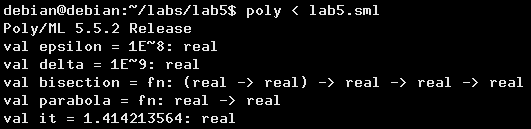
\includegraphics[scale=0.8]{lab5sml.png}
\clearpage
\section{C Code}
We can implement this in C
\begin{GFT}{C source code written to file lab5.c}
\+\#include <stdio.h>\\
\+\#include <math.h>\\
\+const double epsilon = 0.00000001, delta = 0.00000001;\\
\+double parabola(double x) \{return x*x -2.0;\}\\
\+double bisection(double f(double),double low, double high)\\
\+\{\\
\+	double r;\\
\+	double mid = (low+high)/2.0;\\
\+	double image = f(mid);\\
\+	if(fabsl(image) < epsilon) return mid;\\
\+	else if( fabsl(high - low) < delta) return mid;\\
\+	else if (image < 0.0) r = bisection(f,mid,high);\\
\+	else r = bisection(f,low,mid);\\
\+	return r;\\
\+\}\\
\+int main()\\
\+\{\\
\+	printf("\%f\Backslash{}n", bisection(parabola,-1.0,15.0));\\
\+\}\\
\end{GFT}
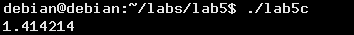
\includegraphics[scale = 0.8]{lab5c.png}
\section{ASM Code}
\subsection{Parabola Function}
\begin{multicols}{2}
\begin{GFT}{asm source code written to file lab5.s}
\+.data\\
\+two: .float 2.0\\
\+.text\\
\+parabola:\\
\+push \%ebp\\
\+mov \%esp, \%ebp\\
\+fld 8(\%ebp) 		\# st0 = x\\
\+fmul 8(\%ebp)		\# st0 = x\Circumflex{}2\\
\+fsub two		\# st0 = x\Circumflex{}2 - 2.0\\
\+mov \%ebp, \%esp\\
\+pop \%ebp\\
\+ret\\
\end{GFT}
\columnbreak
\textit{8(\%ebp)} is your parameter so \textit{fld 8(\%ebp)} will push your parameter to FPU stack. At this point, $st0 = parameter$. \\ \\
Next \textit{fmul 8(\%ebp)} will multiply st0 by your parameter, which means $st0 = parameter^2$. \\ \\
Then \textit{fsub two} will subtract $2.0$ from st0, and $st0 = parameter^2 - 2.0$. We can't do \textit{fsub 2} because the operand for \textit{fsub} just is memory address or register only, that's why we have to create varible \textit{two} to store float value 2.0.
\end{multicols}
\clearpage
\subsection{Bisection Function}
\begin{multicols}{2}
This is the data used in bisection function. The same reason with variable \textit{two} why we create variable \textit{zero} (FPU instruction operand is memory address and register only). We create variable ST0 for storing value from \textit{\%st(0)}, and also for popping unnesscary values in FPU stack.
\begin{GFT}{asm source code appended to file lab5.s}
\+.data\\
\+epsilon: .float 0.000001\\
\+delta: .float 0.000001\\
\+zero: .float 0.0\\
\+ST0: .float 0.0\\
\end{GFT}
Start of bisection function.It will take 3 parameters:
\begin{description}
\item[parabola]  6(\%ebp)
\item[low]  12(\%ebp)
\item[high]  8(\%ebp)
\end{description}
\begin{GFT}{asm source code appended to file lab5.s}
\+.text\\
\+bisection:\\
\+push \%ebp\\
\+mov \%esp, \%ebp\\
\+fld 8(\%ebp) 		\#st0 = high\\
\+fadd 12(\%ebp)		\#st0 = high + low\\
\+fdiv two		\#st0 = (high+low)/2\\
\end{GFT}
First, we create variable \(mid = \frac{high + low}{2}\). We push \textit{high} onto FPU stack, so $st0 = high$ Then add \textit{low} to st0, and divide it by 2. You stack at this time : \\
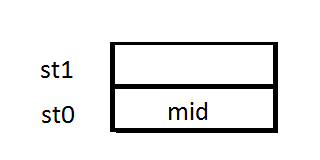
\includegraphics[scale=0.5]{stack1.png} \\
\begin{GFT}{asm source code appended to file lab5.s}
\+fst ST0\\
\+push ST0\\
\+mov 16(\%ebp), \%eax\\
\+call *\%eax 	\\
\+add \$4,\%esp\\
\end{GFT}
The code above creates varible \(image = f(mid)\). We store value from \textit{\%st0 = mid} to variable ST0 by using \textit{fst ST0}, then push ST0 onto stack for calling function. \\ 
We passed memory adress of function parabola to parameter for bisection function: \(\$parabola = 16(\%ebp)\). That's why we copy \textit{16(\%ebp)} into EAX for using \textit{call *\%eax}, which means calling function with address stored in EAX.
\end{multicols}
\pagebreak
\begin{multicols}{2}
After calling function parabola, FPU stack will look like this: \\
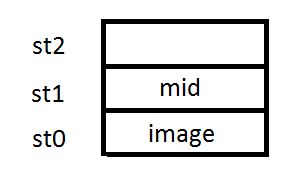
\includegraphics[scale=0.5]{stack2.png} \\
Then we will move to first condition: \\ \\ \textbf{if( fabsl(image) \textless epsilon) return mid;}
\begin{GFT}{asm source code appended to file lab5.s}
\+fld \%st(0)		\# st0 = image	\\
\+fabs			\# st0 = |image|\\
\+fld epsilon		\# st0 = epsilon\\
\+fcomip			\# compare st0 and st1\\
\+\#pop |image| out, st0 =image\\
\+fstp ST0		\#st0 = image, st1= mid\\
\+ja \_end			\# if st0 > st1\\
\end{GFT}
Since we need \textit{image} for later use, we push another \textit{image} onto FPU stack. Then \textit{fabs} will take absolute of st0.\\
To compare floating point number, we use \textit{fcomi} to compare st0 and st1 (st0 will be in left side of expression). \\
\columnbreak
 That's why we push \textit{epsilon} to FPU stack. \\
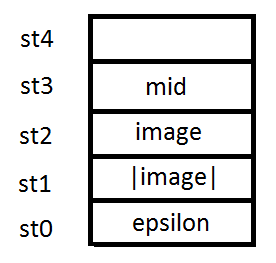
\includegraphics[scale=0.5]{stack3.png} \\
\textit{ja \_end} means that if st0 \textgreater st1, we jump to \textit{\_end} label (end of function). \\ \\
But after comparing, we don't need \textit{epsilon} on FPU stack anymore; hence, we use \textit{fcomip} instead of \textit{fcomi} to pop st0 after comparing $\Rightarrow$ $st0 = |image|$. \\ \\
We also don't need $|iamge|$ on stack, so we pop it out (store to ST0 for temporary). FPU stack after cleaning: \\ \\
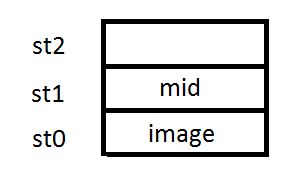
\includegraphics[scale=0.5]{stack2.png} \\
\end{multicols}
\pagebreak
\begin{multicols}{2}
Move to second condition: \\ \\ \textbf{if( fabsl(high-low) \textless delta) return mid;} \\
\begin{GFT}{asm source code appended to file lab5.s}
\+fld 8(\%ebp) 		\#st0 = high\\
\+fsub 12(\%ebp)		\#st0 = high - low\\
\+fabs			\#st0 = |high - low|\\
\+fld delta		\#st0 = delta\\
\+fcomip			\\
\+\#pop |high -low|, st0 =image\\
\+fstp ST0		\#st0 = image, st1= mid\\
\+ja \_end			\# if st0 > st1\\
\end{GFT}
We do the same thing for first condition, push $|high-low|$ instead of $|image|$. Remind you that \textit{8(\%ebp) = high, 12(\%ebp) = low}. Process of stack changing: \\ \\
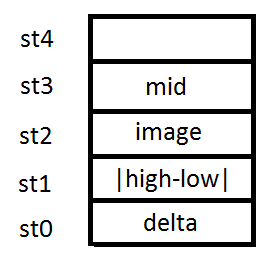
\includegraphics[scale=0.5]{stack4.png}
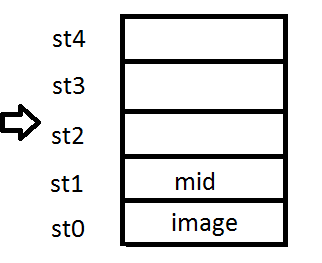
\includegraphics[scale=0.5]{stack5.png} 
\\ \\ 
\columnbreak
\\Move to last two conditions: \\ \\ \textbf{if (image \textless 0.0) r = bisection(f,mid,high);} \\ \\
\textbf{else r = bisection(f,low,mid);} \\
\begin{GFT}{asm source code appended to file lab5.s}
\+fld zero		\# st0 = 0\\
\+fcomip\\
\+fstp ST0		\# pop image, st0 = mid			\\
\+ja \_if			\# if image < 0\\
\end{GFT}
The same thing above, to compare with 0, we push 0 onto stack for using \textit{fcomip}. After compare, 0 is popped out. At this point, we need to clear \textit{image} as well, since we don't need it for later $\Rightarrow$ Doing \textit{fstp ST0} again. \\ \\
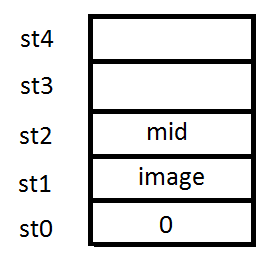
\includegraphics[scale=0.5]{stack6.png}
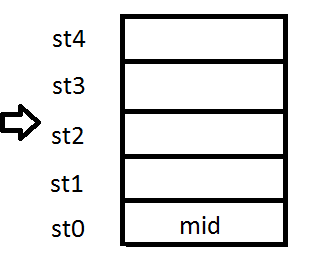
\includegraphics[scale=0.5]{stack7.png} \\
\end{multicols}
\pagebreak
\begin{multicols}{2}
This is \textit{else} part for calling
\begin{center}
\textbf{bisection(f,low,mid)} 
\end{center}
\begin{GFT}{asm source code appended to file lab5.s}
\+push 16(\%ebp)		\# parabola\\
\+push 12(\%ebp)		\# low		\\
\+fstp ST0		\\
\+push ST0		\# mid\\
\+call bisection\\
\+add \$12, \%esp\\
\+jmp \_end\\
\end{GFT}
\columnbreak
This is \textit{if} part for calling 
\begin{center}
\textbf{bisection(f,mid,high)}
\end{center}
\begin{GFT}{asm source code appended to file lab5.s}
\+\_if:\\
\+push 16(\%ebp)		\#parabola\\
\+fstp ST0		\#mid\\
\+push ST0\\
\+push 8(\%ebp)		\#high\\
\+call bisection\\
\+add \$12, \%esp\\
\end{GFT}
\end{multicols}
Since our FPU stack for last time has $st0 = mid$, when we do \textit{fstp ST0}, $ST0$ will be equal to $mid$, then we can go ahead push it on stack for using as parameter. \textit{fstp} is used instead of \textit{fst} because we don't need $mid$ after calling bisection. At this moment, our FPU stack is clear totally. \\ \\ This is the $\_end$ label to end function calling.
\begin{GFT}{asm source code appended to file lab5.s}
\+\_end:\\
\+mov \%ebp, \%esp\\
\+pop \%ebp\\
\+ret\\
\end{GFT}
\clearpage
\subsection{Main function}
\begin{multicols}{2}
Datas used for main only
\begin{GFT}{asm source code appended to file lab5.s}
\+.data\\
\+high: .float 15.0\\
\+low: .float -1.0\\
\+fmt: .string "The root for function f is : \%f\Backslash{}n"\\
\end{GFT}
Start of program, call bisection with 3 parameters: address of parabola, low, high. \\
\begin{GFT}{asm source code appended to file lab5.s}
\+.text\\
\+.globl \_start\\
\+\_start:\\
\+push \$parabola\\
\+push low\\
\+push high\\
\+call bisection\\
\+add \$12, \%esp\\
\+fstp ST0\\
\end{GFT}
Bisection is a recursive function, and remember that the last time of bisection calling inside bisection function will fall into situation either \textit{$|image|$ \textless epsilon} or \textit{$|high - low|$ \textless delta}, which means that after call bisection, our stack: \\ \\
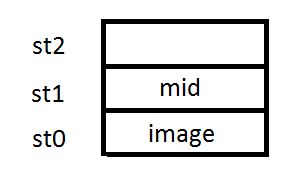
\includegraphics[scale=0.5]{stack2.png} \\ \\
So we need to pop $image$ out because $mid$ is the final answer we need. \\ \\
Since variabel ST0 is just 32-bit and printf need 64-bit floating point, we can't pop value in $st0$ to ST0. Instead, we \textit{add \$-8, \%esp} to create room for 64-bit floating point number that we pop from $st0$ by using $fstpl$ (that's why we \textit{add \$12, \%esp} in the end.)
\begin{GFT}{asm source code appended to file lab5.s}
\+add \$-8, \%esp\\
\+fstpl (\%esp)\\
\+push \$fmt\\
\+call printf\\
\+add \$12, \%esp\\
\end{GFT}
End main function.
\begin{GFT}{asm source code appended to file lab5.s}
\+mov \$1, \%eax\\
\+mov \$0, \%ebx\\
\+int \$0x80\\
\end{GFT}
\end{multicols}
\clearpage
Testing result for ASM code \\ \\
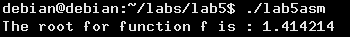
\includegraphics[scale = 0.8]{lab5asm.png} \\
\section{Create build.sh file}
This file is used for building gnuplot and making lab5 pdf. Run \textit{./build.sh} will do all these code in terminal
\begin{GFT}{Text written to file build.sh}
\+docsml lab5.doc\\
\+gnuplot bisectionfig1.gp\\
\+gnuplot bisectionfig2.gp\\
\+doctex lab5.doc\\
\+pptexenv pdflatex lab5.tex\\
\end{GFT}
This command make \textit{buid.sh} executable.
\begin{GFT}{Bourne Shell}
\+chmod 777 build.sh\\
\end{GFT}
\end{document}

